\documentclass[times]{G7-32} % стиль и язык

\sloppy

% Настройки стиля ГОСТ 7-32
% Для начала определяем, хотим мы или нет, чтобы рисунки и таблицы нумеровались в пределах раздела, или нам нужна сквозная нумерация.
\EqInChapter % формулы будут нумероваться в пределах раздела
\TableInChapter % таблицы будут нумероваться в пределах раздела
\PicInChapter % рисунки будут нумероваться в пределах раздела

\renewcommand{\DefinesIntro}{В настоящей выпускной квалификационной работе магистра применяют следующие сокращения и обозначения:}

% Добавляем гипертекстовое оглавление в PDF
\usepackage[
bookmarks=true, colorlinks=true, unicode=true,
urlcolor=black,linkcolor=black, anchorcolor=black,
citecolor=black, menucolor=black, filecolor=black,
]{hyperref}

\AfterHyperrefFix

\usepackage{microtype}% полезный пакет для микротипографии, увы под xelatex мало чего умеет, но под pdflatex хорошо улучшает читаемость

% Тире могут быть невидимы в Adobe Reader
\ifInvisibleDashes
\MakeDashesBold
\fi

\usepackage{graphicx}   % Пакет для включения рисунков

% С такими оно полями оно работает по-умолчанию:
% \RequirePackage[left=20mm,right=10mm,top=20mm,bottom=20mm,headsep=0pt,includefoot]{geometry}
% Если вас тошнит от поля в 10мм --- увеличивайте до 20-ти, ну и про переплёт не забывайте:
\geometry{right=15mm}
\geometry{left=30mm}
\geometry{bottom=20mm}
\geometry{ignorefoot}% считать от нижней границы текста


% Пакет Tikz
\usepackage{tikz}
\usetikzlibrary{arrows,positioning,shadows}

% Произвольная нумерация списков.
\usepackage{enumerate}

% ячейки в несколько строчек
\usepackage{multirow}

% itemize внутри tabular
\usepackage{paralist,array}

%\setlength{\parskip}{1ex plus0.5ex minus0.5ex} % разрыв между абзацами
\setlength{\parskip}{1ex} % разрыв между абзацами
\usepackage{blindtext}

% Центрирование подписей к плавающим окружениям
%\usepackage[justification=centering]{caption}

\usepackage{newfloat}
\DeclareFloatingEnvironment[
placement={!ht},
name=Equation
]{eqndescNoIndent}
\edef\fixEqndesc{\noexpand\setlength{\noexpand\parindent}{\the\parindent}\noexpand\setlength{\noexpand\parskip}{\the\parskip}}
\newenvironment{eqndesc}[1][!ht]{%
    \begin{eqndescNoIndent}[#1]%
\fixEqndesc%
}
{\end{eqndescNoIndent}}
 % остальные стандартные настройки убраны в preamble.inc.tex
% Математика
\usepackage{mathtools, cancel, physics, euscript, xfrac, amsmath, amsthm}

\newtheorem{Th}{Теорема}
\newtheorem{Lm}{Лемма}
\newtheorem{Df}{Определение}
\newtheorem{Ex}{Пример}
\newtheorem{Rm}{Ремарка}
\newtheorem{Alg}{Алгоритм}
\newtheorem{Ax}{Аксиома}
\newtheorem{Crl}{Следствие}
\newtheorem{Prp}{Гипотеза}


% Настройки листингов.
\ifPDFTeX
% 8 Листинги

\usepackage{listings}

% Значения по умолчанию
\lstset{
  basicstyle= \footnotesize,
  breakatwhitespace=true,% разрыв строк только на whitespacce
  breaklines=true,       % переносить длинные строки
%   captionpos=b,          % подписи снизу -- вроде не надо
  inputencoding=koi8-r,
  numbers=left,          % нумерация слева
  numberstyle=\footnotesize,
  showspaces=false,      % показывать пробелы подчеркиваниями -- идиотизм 70-х годов
  showstringspaces=false,
  showtabs=false,        % и табы тоже
  stepnumber=1,
  tabsize=4,              % кому нужны табы по 8 символов?
  frame=single
}

% Стиль для псевдокода: строчки обычно короткие, поэтому размер шрифта побольше
\lstdefinestyle{pseudocode}{
  basicstyle=\small,
  keywordstyle=\color{black}\bfseries\underbar,
  language=Pseudocode,
  numberstyle=\footnotesize,
  commentstyle=\footnotesize\it
}

% Стиль для обычного кода: маленький шрифт
\lstdefinestyle{realcode}{
  basicstyle=\scriptsize,
  numberstyle=\footnotesize
}

% Стиль для коротких кусков обычного кода: средний шрифт
\lstdefinestyle{simplecode}{
  basicstyle=\footnotesize,
  numberstyle=\footnotesize
}

% Стиль для BNF
\lstdefinestyle{grammar}{
  basicstyle=\footnotesize,
  numberstyle=\footnotesize,
  stringstyle=\bfseries\ttfamily,
  language=BNF
}

% Определим свой язык для написания псевдокодов на основе Python
\lstdefinelanguage[]{Pseudocode}[]{Python}{
  morekeywords={each,empty,wait,do},% ключевые слова добавлять сюда
  morecomment=[s]{\{}{\}},% комменты {а-ля Pascal} смотрятся нагляднее
  literate=% а сюда добавлять операторы, которые хотите отображать как мат. символы
    {->}{\ensuremath{$\rightarrow$}~}2%
    {<-}{\ensuremath{$\leftarrow$}~}2%
    {:=}{\ensuremath{$\leftarrow$}~}2%
    {<--}{\ensuremath{$\Longleftarrow$}~}2%
}[keywords,comments]

% Свой язык для задания грамматик в BNF
\lstdefinelanguage[]{BNF}[]{}{
  morekeywords={},
  morecomment=[s]{@}{@},
  morestring=[b]",%
  literate=%
    {->}{\ensuremath{$\rightarrow$}~}2%
    {*}{\ensuremath{$^*$}~}2%
    {+}{\ensuremath{$^+$}~}2%
    {|}{\ensuremath{$|$}~}2%
}[keywords,comments,strings]

% Подписи к листингам на русском языке.
\renewcommand\lstlistingname{Листинг}
\renewcommand\lstlistlistingname{Листинги}

\else
\usepackage{local-minted}
\fi

% Любимые команды
\newcommand{\Code}[1]{\textbf{#1}}
 % полезные макросы листингов


%\NirEkz{Экз. 3}                                  % Раскоментировать если не требуется
%\NirGrif{Секретно}                % Наименование грифа

%\gosttitle{Gost7-32}       % Шаблон титульной страницы, по умолчанию будет ГОСТ 7.32-2001, 
% Варианты GostRV15-110 или Gost7-32 
 
\NirOrgLongName{Министерство общего и профессионального образования \\
Российской Федерации\par
ГОСУДАРСТВЕННЫЙ ТЕХНИЧЕСКИИ УНИВЕРСИТЕТ
}                                           %% Полное название организации

% \NirUdk{УДК № 378.14}
% \NirGosNo{№ госрегистрации 01970006723}
%\NirInventarNo{Инв. № ??????}

%\NirConfirm{Согласовано}                  % Смена УТВЕРЖДАЮ
\NirBoss[.49]{Проректор университета\\по научной работе}{И.И. Иванов}            %% Заказчик, утверждающий НИР


%\NirReportName{Научно-технический отчет}   % Можно поменять тип отчета
%\NirAbout{О составной части \par опытно-конструкторской работы} %Можно изменить о чем отчет

%\NirPartNum{Часть}{1}                      % Часть номер

%\NirBareSubject{}                  % Убирает по теме если раскоментить

% \NirIsAnnotacion{АННОТАЦИОННЫЙ }         %% Раскомментируйте, если это аннотационный отчёт
%\NirStage{промежуточный}{Этап \No 1}{} %%% Этап НИР: {номер этапа}{вид отчёта - промежуточный или заключительный}{название этапа}
%\NirStage{}{}{} %%% Этап НИР: {номер этапа}{вид отчёта - промежуточный или 

\Nir{Социально-экономические проблемы подготовки военных специалистов\\в гражданских вузах России}

\NirSubject{ФЕМИНИЗАЦИЯ АРМИИ КАК СОЦИАЛЬНЫЙ ПРОЦЕСС}                                   % Наименование темы
%\NirFinal{}                        % Заключительный, если закоментировать то промежуточный
%\finalname{итоговый}               % Название финального отчета (Заключительный) 
%\NirCode{Шифр\,---\,САПР-РЛС-ФИЗТЕХ-1} % Можно задать шифр как в ГОСТ 15.110
\NirCode{}

\NirManager{Зам. проректора по научной работе}{И.И. Иванов} %% Название руководителя
\NirIsp{Руководитель темы}{И.И. Иванов} %% Название руководителя

\NirYear{2024}%% если нужно поменять год отчёта; если закомментировано, ставится текущий год
\NirTown{Москва}                           %% город, в котором написан отчёт
 % стиль титульного листа и заголовки

\begin{document}

\frontmatter % выключает нумерацию ВСЕГО; здесь начинаются ненумерованные главы: реферат, введение, глоссарий, сокращения и прочее.

\maketitle % создает титульную страницу

\begin{executors}
    \personalSignature{Первый исполнитель}{ФИО}
    \personalSignature{Второй исполнитель}{ФИО}
\end{executors}

%\listoffigures % список рисунков

%\listoftables % список таблиц

%\NormRefs % нормативные ссылки 
% Команды \breakingbeforechapters и \nonbreakingbeforechapters
% управляют разрывом страницы перед главами.
% По-умолчанию страница разрывается.

% \nobreakingbeforechapters
% \breakingbeforechapters

\Referat

Отчет \pageref{LastPage}\,стр.%
\ifnum \totfig >0
, \totfig~рис.%
\fi
\ifnum \tottab >0
, \tottab~табл.%
\fi
%
\ifnum \totbib >0
, \totbib~источн.%
\fi
%
\ifnum \totapp >0
, \totapp~прил.%
\else
% .%
\fi

\noindent
ЭЛЕКТРОНИКА, ИНФОРМАЦИОННЫЕ ТЕХНОЛОГИИ, USB 2.0, ULPI, TTL, RGB, RGBI, ПЛИС, VHDL, КАДРОВЫЙ БУФЕР, PSRAM, ДИСПЛЕЙ

Объектом исследования является протокол ULPI и способы применения интерфейса USB для передачи видеоданных.

Цель работы: разработка заказного устройства отображения на базе ПЛИС.

В ходе НИР были получены следующие результаты:

\begin{enumerate}
\longitem{Предложена структура устройства отображения, описаны его составные части}
\longitem{Рассмотрена работа устройства отображения}
\longitem{Разработаны необходимые алгоритмы для устройства отображения}
\finalitem{Произведена верификация и реализация устройства отображения}
\end{enumerate}


\tableofcontents

\printnomenclature % автоматический список сокращений

\Introduction

Добавлять пункты в "{}Термины и определения"{} и "{}Перечень сокращений и обозначений"{} можно где угодно в коде. Команда \verb|\Define| добавляет пункт в первый список, \verb|\Abbrev| добавляет пункт во второй список. 

Проверяем как у нас работают сокращения, обозначения и определения "---
MAX,
\Abbrev{MAX}{maximum "--- максимальное значение параметра}
API
\Abbrev{API}{application programming interface "--- внешний интерфейс взаимодействия с приложением}
с обратным прокси.
\Define{Обратный прокси}{тип прокси-сервера, который ретранслирует}


\mainmatter % это включает нумерацию глав и секций в документе ниже

\chapter{Аналитический раздел}
\label{cha:analysis}


В данном разделе анализируется и классифицируется существующая всячина и рассматриваются способы создания новой всячины.

\section{Анализ того и сего}

В работе можно использовать разделы \verb|\chapter|, \verb|\section|, подразделы \verb|\subsection|, подподраздела \verb|\subsubsection| и параграфа \verb|\paragraph|. Однако, следует помнить, что разделы разрешены только в основной части работы. Во введении, заключении и других структурных элементах они запрещены. Старайтесь избегать случаев, когда в разделе существует только один подраздел.

\subsection{Пример использования подраздела}
\subsubsection{Пример использования подподраздела}

\paragraph{Проверка} параграфа. Вроде работает.
\paragraph{Вторая проверка} параграфа. Опять работает.

\begin{itemize}
\item Это список с палочками. 
\item Хотя он соответствует требованиям ГОСТ, лучше использовать список с номерами, чтобы облегчить чтение.
\end{itemize}

\subsection{Пример использования блок-схемы}

\subsubsection*{Заголовки разделов}

В работе можно использовать и подподпункты, например \verb|\subsubsection|. Однако, лучше не нумеровать этот уровень разделов, чтобы не усложнять структуру документа.

\section{Подсистема всякой ерунды}

Существует несколько подсистем, среди которых можно выделить:

\begin{enumerate}
\item Перечисление с номерами.
\item Нумерация первого уровня. В соответствии с ГОСТ, первый уровень нумеруется буквами, а на втором уровне "--- цифрами. Элементы на первом уровне выравниваются как обычные абзацы. Проверим теперь вложенные списки.
\begin{enumerate}
\item Нумерация второго уровня.
\item Нумерация второго уровня. Проверяем на очень длинной строке, чтобы убедиться, что выравнивание работает правильно.
\end{enumerate}
\item По мнению Лукьяненко, человеческий мозг старается свести любую проблему к выбору из трех вариантов.
\item Четвертый (и последний) элемент списка.
\end{enumerate}

\chapter{Конструкторский раздел}
\label{cha:design}

В этом разделе описан состав, структура и алгоритмы работы устройства отображения в виде конечных автоматов.

\section{Структура устройства отображения}

Структурная схема работы устройства отображения показана на рисунке \ref{fig:structure}.

\begin{figure}[ht]
    \centering
    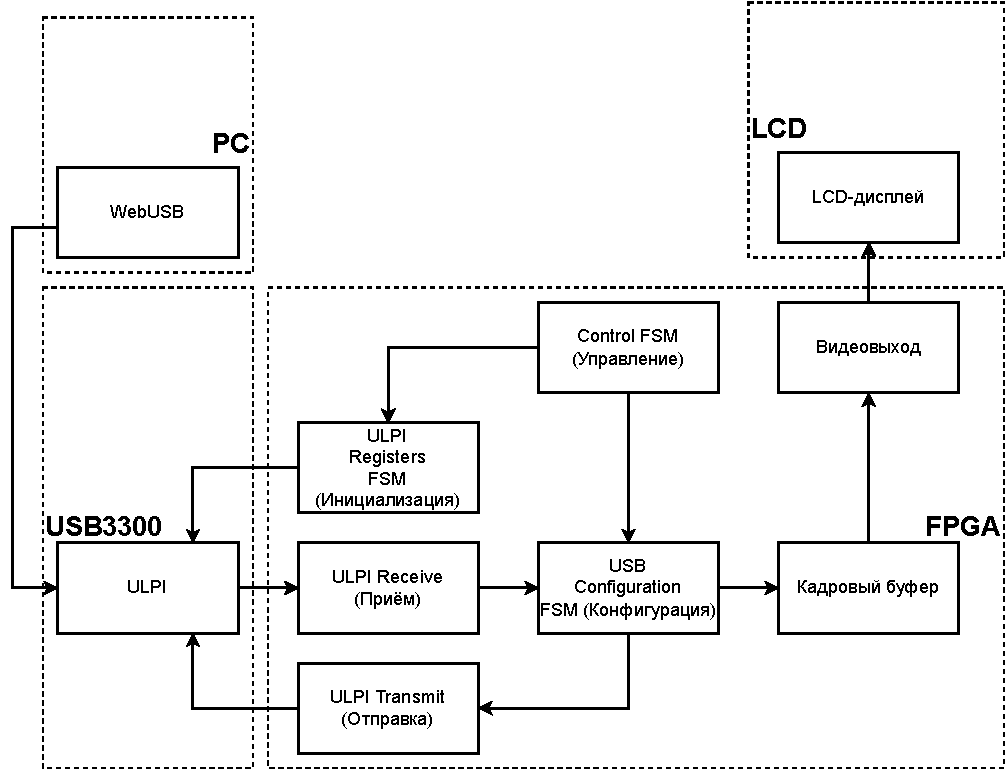
\includegraphics[scale=0.7]{res/img/structure.pdf}
    \caption{Структурная схема устройства отображения}
    \label{fig:structure}
\end{figure}

При запуске устройства происходит его инициализация. Затем ПК проводит опрос устройства, в ответ оно отправляет свои конфигурационные дескрипторы. После этого устройство считается сконфигурированным.

При помощи программы передачи изображения происходит отправка кадров устройству, сохраняющими их в кадровом буфере. Видеовыход вычитывает текущий кадр из буфера и отображает его на дисплее.

\section{Алгоритм работы устройства управления}

На рисунке \ref{fig:fsm_control_state} представлен конечный автомат блока управления. Устройство начинает с инициализации ULPI, после чего ожидает подключения USB интерфейса. Как только интерфейс будет сконфигурирован, блок управления будет ожидать отключения устройства. После отключения автомат вернётся в состояние ожидания подключения устройства.

\begin{figure}[ht]
    \centering
    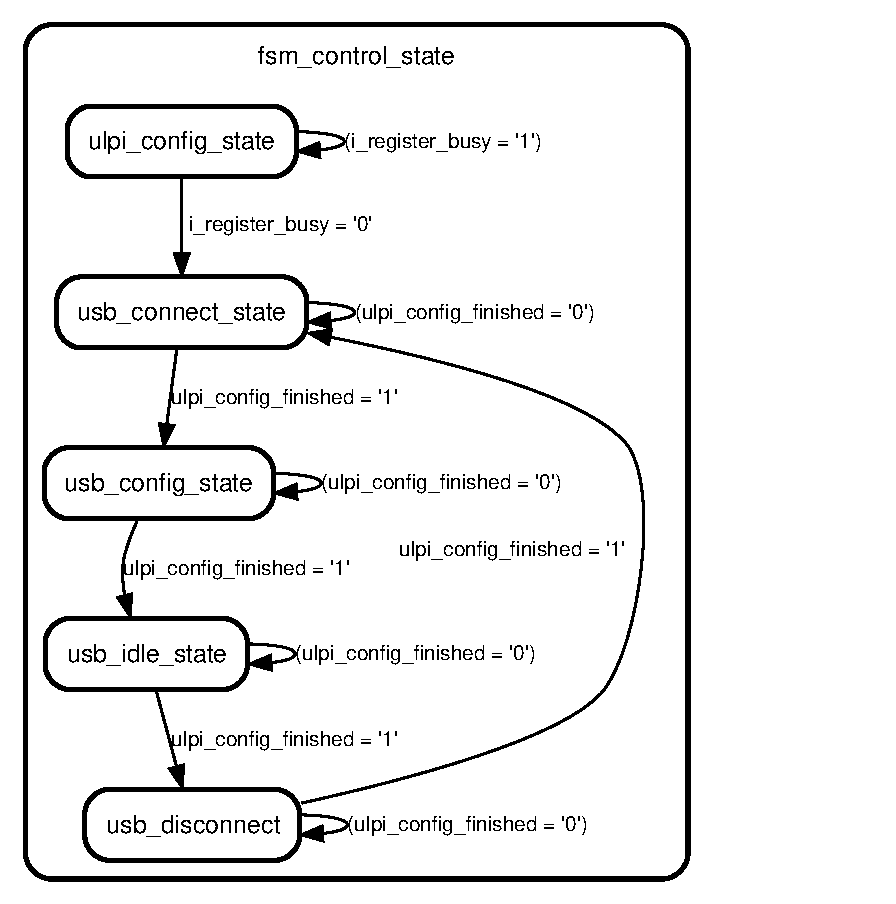
\includegraphics[scale=1]{res/img/fsm_control_state.pdf}
    \caption{Конечный автомат блока управления}
    \label{fig:fsm_control_state}
\end{figure}

\section{Алгоритм работы блока конфигурации}

Блок конфигурации обрабатывает сообщения протокола USB, поступающие от ПК, и формирует на них ответ. Его конечный автомат представлен на рисунке \ref{fig:fsm_usb_config_state}.

\begin{figure}[ht]
    \centering
    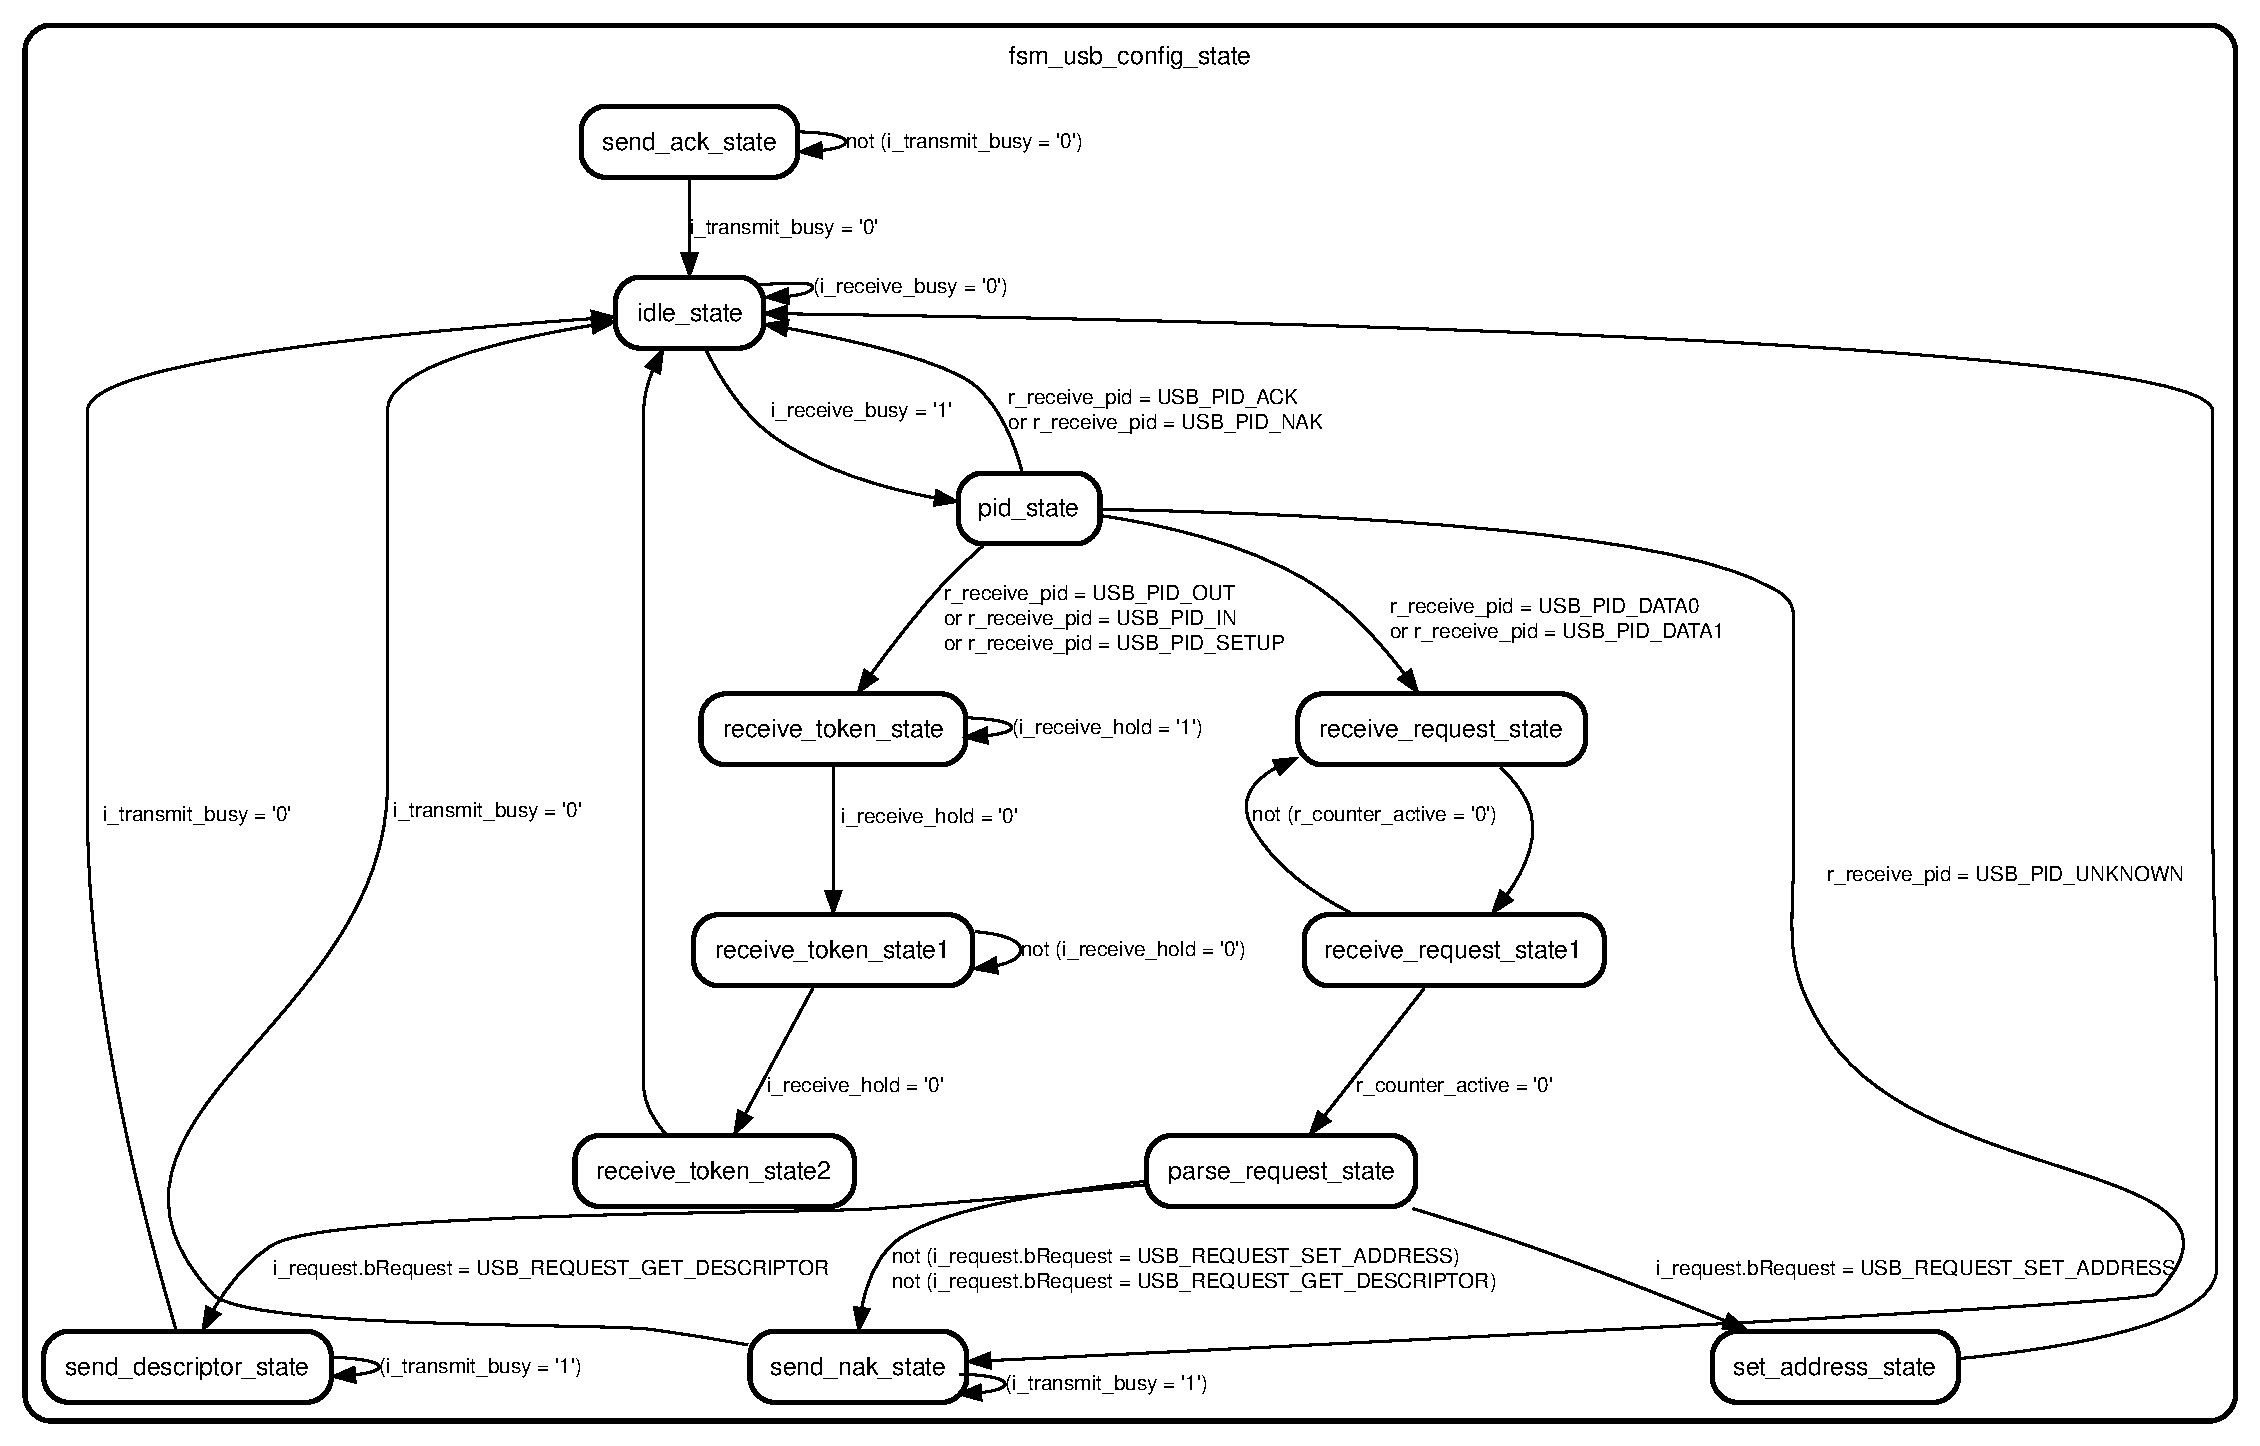
\includegraphics[scale=0.45]{res/img/fsm_usb_config_state.pdf}
    \caption{Конечный автомат блока конфигурации}
    \label{fig:fsm_usb_config_state}
\end{figure}

Конфигурация происходит в следующем порядке:

% \begin{enumerate}
\begin{enumerate}
\item ПК начинает транзакцию SETUP;
\item ПК запрашивает дескриптор устройства;
\item Устройство отвечает дескриптором;
\item ПК вновь начинает транзакцию SETUP;
\item ПК устанавливает адрес устройства;
\item Устройство принимает адрес и подтверждает;
\item ПК повторяет запрос дескриптора с новым адресом;
\item Устройство отправляет дескриптор;
\item ПК подтверждает принятие дескриптора и завершает транзакцию;
\item Устройство подтверждает завершение транзакции.
\end{enumerate}
% \end{enumerate}

\section{Алгоритм работы блока инициализации}

Блок инициализации записывает или считывает (в зависимости от команды) параметры из регистров ULPI. Его конечный автомат представлен на рисунке \ref{fig:fsm_ulpi_registers_state}.

\begin{figure}[ht]
    \centering
    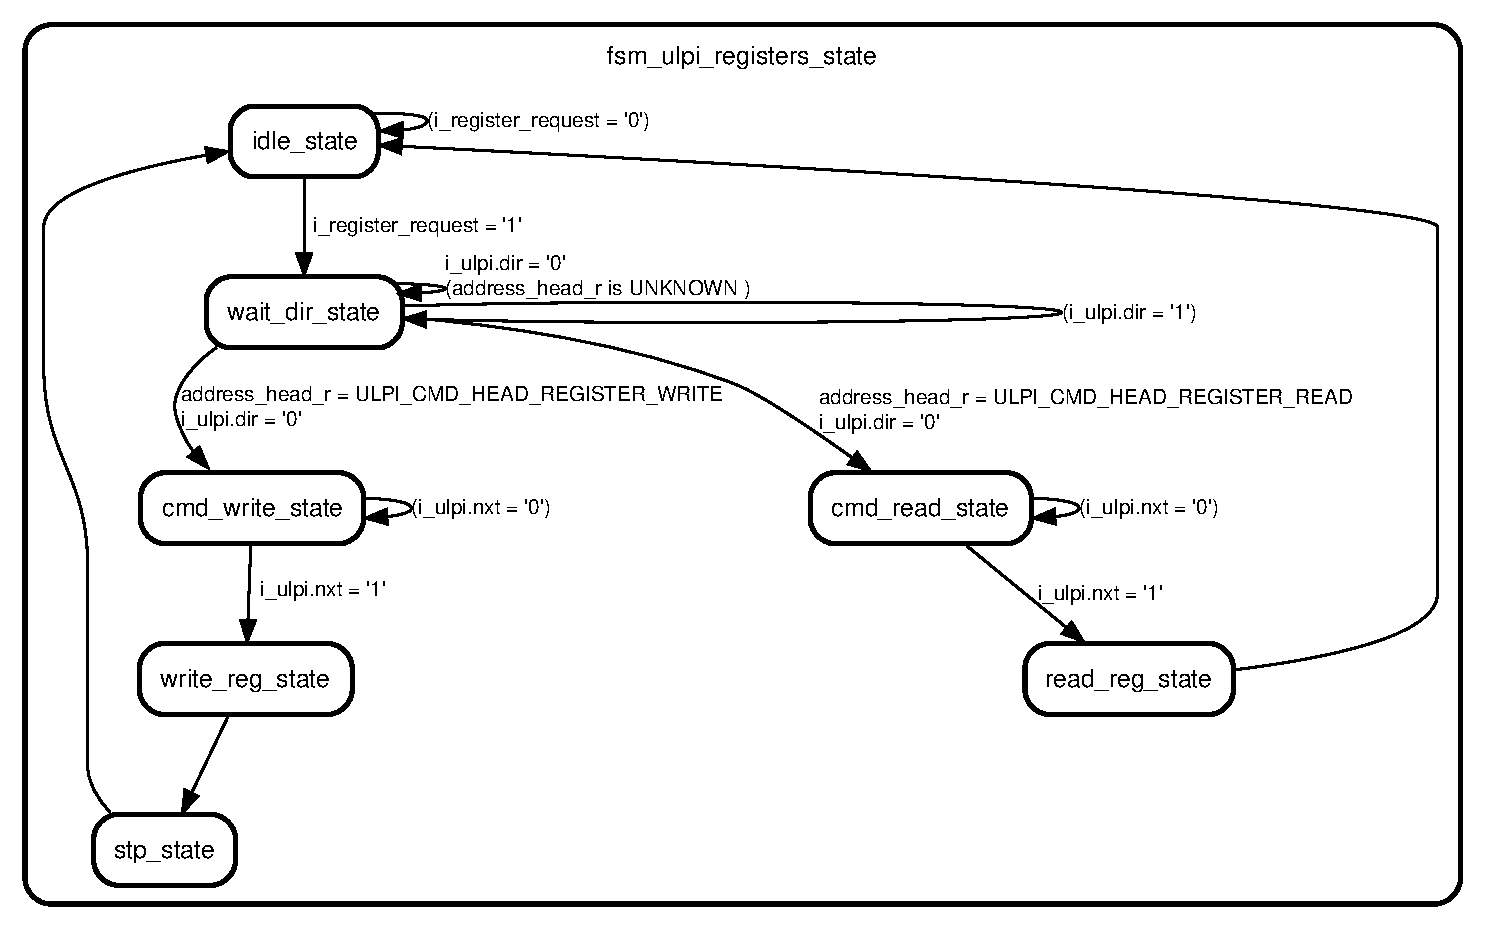
\includegraphics[scale=0.6]{res/img/fsm_ulpi_registers_state.pdf}
    \caption{Конечный автомат блока инициализации}
    \label{fig:fsm_ulpi_registers_state}
\end{figure}

\section{Выводы}

% \begin{enumerate}
\begin{enumerate}
\item Описана структура устройства отображения, выделены его составные части.
\item Описаны алгоритмы работы блоков в виде конечных автоматов.
\item Описан порядок конфигурации устройства в блоке конфигурации.
% \end{enumerate}
\end{enumerate}

\chapter{ВЕРИФИКАЦИЯ И РЕАЛИЗАЦИЯ УСТРОЙСТВА}
\label{cha:impl}

В данном разделе будет представлена практическая часть НИР, а именно верификация работы и реализация цифровой схемы устройства на ПЛИС.

\section{Верификация}

Для моделирования работы системы было реализовано тестовое окружение для формирования тестовых воздействий на модули управления устройства. При помощи системы моделирования Questa Sim были построены временные диаграммы работы устройства. На рисунке \ref{fig:verification_all} показан общий вид временной диаграммы.


\begin{figure}[ht]
    \centering
    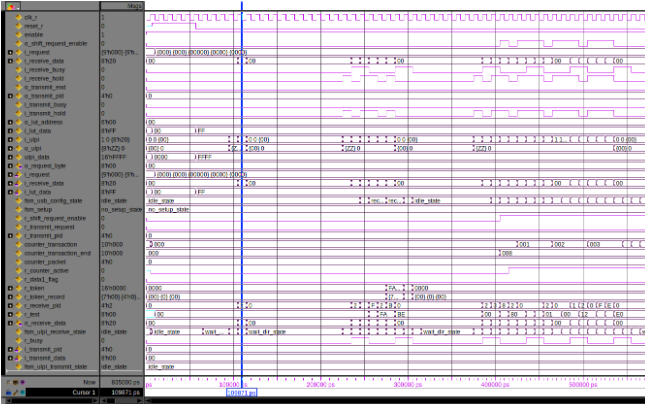
\includegraphics[scale=0.7]{res/img/verification_all.png}
    \caption{Общий вид временной диаграммы}
    \label{fig:verification_all}
\end{figure}

\pagebreak
На рисунке \ref{fig:verification_setup} представлена диаграмма отправки токена SETUP на модуль блока конфигурации. Данные помещаются в регистры, соответствующие их назначению в протоколе: сравниваются адрес, конечная точка и контрольная сумма CRC5. Модуль корректно обрабатывает задержки со стороны устройства при установке \detokenize{i_ulpi.nxt} в логический 0. При этом вход двунаправленной шины данных помещается в высокоимпедансное состояние Z для избежания конфликтов на шине.

\begin{figure}[ht]
    \centering
    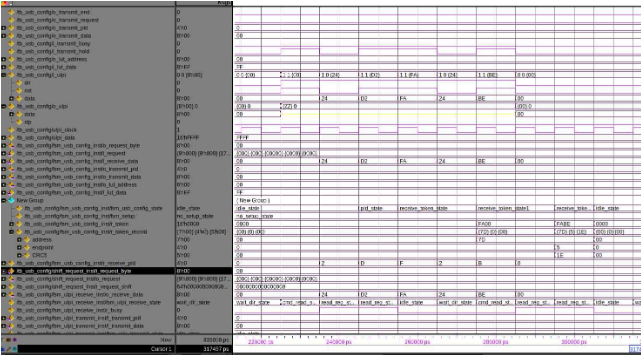
\includegraphics[scale=0.7]{res/img/verification_setup.png}
    \caption{Диаграмма отправки токена SETUP}
    \label{fig:verification_setup}
\end{figure}

\pagebreak
На рисунке \ref{fig:verification_data0} изображена диаграмма передачи длинного сообщения DATA0.

\begin{figure}[ht]
    \centering
    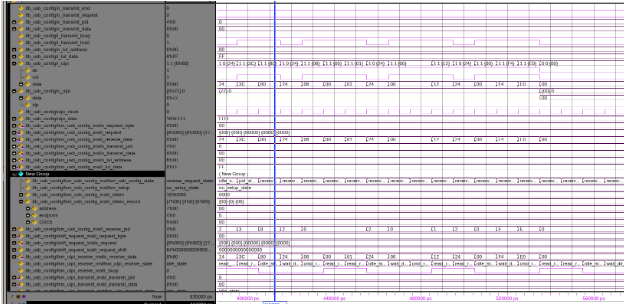
\includegraphics[scale=0.7]{res/img/verification_data0.png}
    \caption{Диаграмма отправки токена DATA0}
    \label{fig:verification_data0}
\end{figure}

На рисунке \ref{fig:verification_ack} изображена диаграмма передачи короткой квитанции ACK подтверждения сообщения.


\begin{figure}[ht]
    \centering
    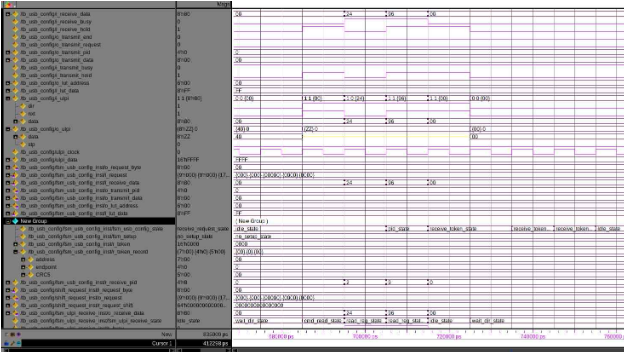
\includegraphics[scale=0.7]{res/img/verification_ack.png}
    \caption{Диаграмма отправки токена ACK}
    \label{fig:verification_ack}
\end{figure}


\section{Практическая реализация}

Был выполнен синтез проекта на ПЛИС GoWin GW1NR-9 в среде GoWin EDA. На рисунке \ref{fig:synth_report} представлены результаты проведённого синтеза и отчёт о занимаемых ресурсах. Все этапы синтеза пройдены успешно. На рисунке \ref{fig:synth_rtl} показана синтезированная схема модуля.

\begin{figure}[ht!]
    \centering
    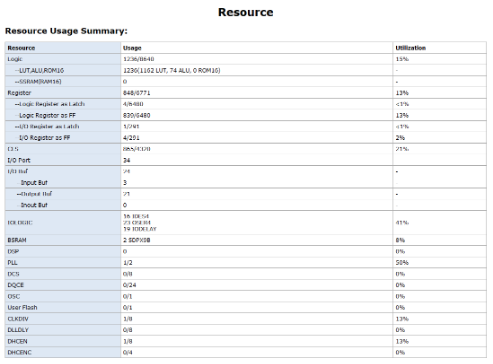
\includegraphics[scale=0.7]{res/img/synth_report.png}
    \caption{Отчёт о занимаемых ресурсах}
    \label{fig:synth_report}
\end{figure}


\begin{figure}[ht!]
    \centering
    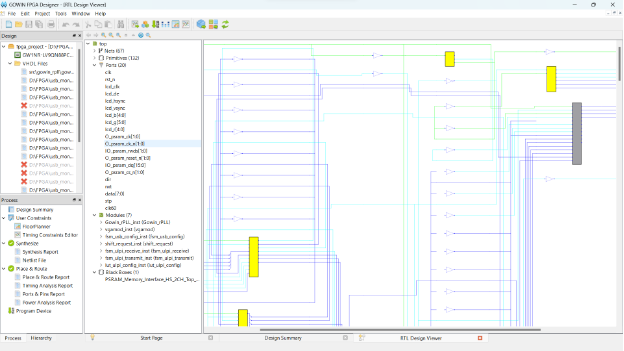
\includegraphics[scale=0.7]{res/img/synth_rtl.png}
    \caption{Синтезируемая схема модуля}
    \label{fig:synth_rtl}
\end{figure}

\begin{figure}[ht!]
    \centering
    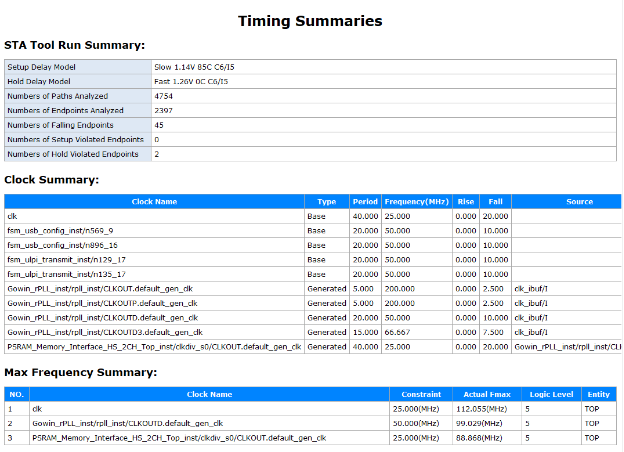
\includegraphics[scale=0.7]{res/img/synth_timing.png}
    \caption{Отчёт о временных характеристиках модуля}
    \label{fig:synth_timing}
\end{figure}



Временных характеристик искомой ПЛИС оказалось достаточно для реализации данного проекта, все временные требования к тактовым сигналам и делителям частоты были соблюдены, что отражено в отчёте, отображённом на рисунке \ref{fig:synth_timing}.

\chapter{Экспериментальный раздел}
\label{cha:research}

Математическая формула может встречаться в тексте: $E = mc^2$. Для больших формул следует использовать окружение \verb|equation|:
\begin{equation}\label{eq:f1}
    E = mc^2.
\end{equation}
На формулу можно сослаться, например, так: (\ref{eq:f1}). См. также раздел \ref{cha:econom}. Использование других окружений для формул, таких как двойные доллары или скобки:
\[
    E = mc^2,
\]
не рекомендуется из-за отсутствия нумерации.

В конце больших формул следует ставить подходящий знак препинания в соответствии с контекстом: точку, запятую, точку с запятой или ничего.

Согласно ГОСТ, каждое новое обозначение, вводимое в формуле, должно быть пояснено сразу после неё. Например:
\begin{equation}
    E = mc^2,
\end{equation}
где $m$ "--- масса, $c$ "--- скорость света.

Несколько примеров:

Формула с текстом:
\begin{equation}
    50 \text{ яблок} \times 100 \text{ яблок} =
    \textbf{ много яблок}
\end{equation}

Различные буквы и шрифты:
\begin{equation}
    \alpha,  \beta,  \gamma, \Gamma, \pi, \Pi, \phi, \varphi, \mu, \Phi, \xi, \zeta;
\end{equation}
\begin{equation}
    \mathbf M, \mathcal C, \mathbb R, \sin \theta = \mathrm{sin} \theta.
\end{equation}

Скобки:
\begin{equation}
    ( a ), [ b ], \{ c \}, | d |, \| e \|, \langle f \rangle, \lfloor g \rfloor, \lceil h \rceil, \ulcorner i \urcorner;
\end{equation}
\begin{equation}
    \left( a + b \right) \left[ 1 - \frac{b}{a+b} \right] = a;
\end{equation}
\begin{equation}
    \sqrt{|xy|} \leq \left| \frac{x + y}{2} \right|;
\end{equation}
\begin{equation}
    \int_a^b u \dv[2]{v}{x} \dd x = \left. u \dv{v}{x} \right|_a^b -\int_a^b \dv{u}{x} \dv{v}{x} \dd x;
\end{equation}
\begin{equation}
    \tilde f(\omega) = \frac{1}{2\pi} \int_{-\infty}^\infty f(x)e^{-i\omega x} \dd x;
\end{equation}
\begin{equation}
    \dot{\vec \omega} = \vec r_c \times \vec I;
\end{equation}
\begin{equation}
    u = \frac{-y}{x^2 + y^2}, \quad v = \frac{x}{x^2 + y^2}, \quad \text{и} \quad w = 0.
\end{equation}

Последовательности:
\begin{equation}
    (1+x)^n = \sum_{i=0}^n \binom{n}{i} x^i;
\end{equation}
\begin{equation}
    e^x = 1 + x + \frac{x^2}{2} + \frac{x^3}{6} + \cdots = \sum_{n \ge 0} \frac{x^n}{n!};
\end{equation}

Дроби:
\begin{equation}
    x = 
    a_0 + \frac{1}{a_1 + \frac{1}{a_2 + \frac{1}{a_3 + a_4}}}
    =
    a_0 + \frac{1}{\displaystyle a_1
        + \frac{1}{\displaystyle a_2
        + \frac{1}{\displaystyle a_3 + a_4}}}.
\end{equation}

Матрицы:
\begin{equation}
    \begin{pmatrix}
        1 & x & 0 \\
        0 & 1 & -1
    \end{pmatrix}
    \begin{pmatrix}
        1  \\
        y  \\
        1
    \end{pmatrix}
    =
    \begin{pmatrix}
        1 + xy  \\
        y - 1
    \end{pmatrix},
    \quad\quad
    \left(
    \begin{matrix}
        2 & 3 & 4\\
        5 & 6 & 7\\
        8 & 9 & 10
    \end{matrix}
    \right)
    v = 0;
\end{equation}
\begin{equation}
    \frac{n!}{k!(n-k)!} = \binom{n}{k};
\end{equation}
\begin{equation}
    \deg A =
    \left|
    \begin{matrix}
        -2 & 1 & 0 & 0 & \cdots & 0  \\
        1 & -2 & 1 & 0 & \cdots & 0  \\
        0 & 1 & -2 & 1 & \cdots & 0  \\
        0 & 0 & 1 & -2 & \ddots & \vdots \\
        \vdots & \vdots & \vdots & \ddots & \ddots & 1  \\
        0 & 0 & 0 & \cdots & 1 & -2
    \end{matrix}
    \right|.
\end{equation}

Фигурная скобка для нескольких случаев:
\begin{equation}
    |x| =
    \begin{cases}
        x, & x \ge 0, \\
        -x, & x< 0.
    \end{cases}
\end{equation}

Формулы в несколько строк:
\begin{align}
    F &= \{ F_{x} \in F_{c} \mid (|S| > |C|) \\
      &\wedge (\mathrm{minPixels} < |S| < \mathrm{maxPixels}) \\
      &\wedge (|S_{\mathrm{conected}}| > |S| - \epsilon) \}
\end{align}
или
\begin{multline}
    A_0 = \frac{1}{(\alpha + t_x)^{r + s + x}}{}_2 F_1 \left( r + s + x, x + 1; r + s + x + 1; \frac{\alpha - \beta}{\alpha + t_x} \right) \\
    \quad - \frac{1}{(\alpha + T)^{r + s + x}}{}_2 F_1 \left( r + s + x, x + 1; r + s + x + 1; \frac{\alpha - \beta}{\alpha + T} \right).
\end{multline}

Логика, доказательства:
\begin{equation}
    (\forall \varepsilon > 0) (\exists N \in \mathbb Z^+) (\forall n \ge N) (|x_n - a| < \varepsilon \iff \lim_{n \to +\infty} x_n = a);
\end{equation}
\begin{equation}
    A \implies B, \quad A \iff B, \quad A = \{z \in \mathbb Z \mid z = \bar z \};
\end{equation}
\begin{equation}
    f: X \to Y, \quad f: x \overset{F}{\mapsto} 5x \cos(\tfrac{\pi x}{2})
\end{equation}
\begin{equation}
    \frac{\cancel{\sqrt 2} \sin(x + 2)}{\cancel{2 \cdot \cos(\sfrac{\pi}{4})} \sin(x)} = \frac{\sin(x + 2)}{\sin(x)}, \quad \cancelto{0}{\sin(0)} \equiv 0.
\end{equation}

\section{Определения и теоремы}

В ГОСТе не представлены инструкции по оформлению определений и теорем. Однако в мировой практике принято следующее стилевое решение, которое можно использовать и в дипломной работе:

\begin{Df}[Метрическое пространство]\label{df:example}
    Метрическим пространством называют пару $(S; \rho)$, где для функции-\textit{метрики} $\rho: S \to \mathbb R^+$, если верно следующие три условия:
    \begin{enumerate}
        \item $a \in S : \rho(a, a) = 0$,
        \item $a, b \in S : \rho(a, b) = \rho(b, a)$,
        \item $a, b, c \in S : \rho(a, b) + \rho(b, c) \ge \rho(a, c)$.
    \end{enumerate}
\end{Df}

\begin{Th}[Хаусдорф]\label{th:example}
    В полном метрическом пространстве множество является компактом тогда и только тогда, когда оно замкнуто и вполне ограничено.
\end{Th}
\begin{proof}
    Текст доказательства.
\end{proof}

\begin{Ex}
    Множество вещественных чисел $\mathbb R$ с заданной на нём метрикой $\rho(a, b) = |a - b|$ формируют метрическое пространство.
\end{Ex}
\begin{proof}
    Следует из определения \ref{df:example}.
\end{proof}

Аналогично картинкам и таблицам, на определения, теоремы и другие блоки можно ссылаться при помощи команды \verb|\ref|: например, на теорему \ref{th:example}.

\chapter{Организационно-экономический раздел}
\label{cha:econom}

Интернет-ссылки оформляются как \url{https://www.google.com/}. Ссылка на картинку, формулу и другие объекты происходит при помощи команды \verb|\ref|: см. рис. \ref{fig:example_fig_1}. На ссылку можно кликнуть и перейти к объекту, на который она ссылается. Ссылка может быть как до объекта, так и после него. Обычно, для удобства, идентификатор начинают с префикса <<\verb|fig:|>> для рисунков, <<\verb|tab:|>> для таблиц, <<\verb|eq:|>> для формул, для <<\verb|section:|>> для разделов, <<\verb|th:|>> для теорем и так далее. Пример ссылки на раздел: см. раздел \ref{cha:research}. 

По условиям ГОСТ-а, на каждую картинку и таблицу должна присутствовать в тексте хотя бы одна ссылка. Желательно рядом с картинкой. Ссылка должна быть оформлена в духе "{}В соответствии с рисунком (таблицей, разделом) 2"{}.

Информация об цитируемых источниках хранится в файлах формата \verb|*.bib|. В этом проекте есть пример такого файла \verb|references.bib|. Похож на формат \verb|json|, но им не является. Заполняйте как можно больше полей там. Сразу готовую запись можно получить прямо в Google Scholar или, часто, на страницах статей на других ресурсах (см. рис. \ref{fig:scholar}). Описание статей начинается с заголовка \verb|@article|, для источников других видов предусмотрены другие заголовки, например \verb|@online| для интернет-страниц.

\begin{figure}[ht]
    \centering
    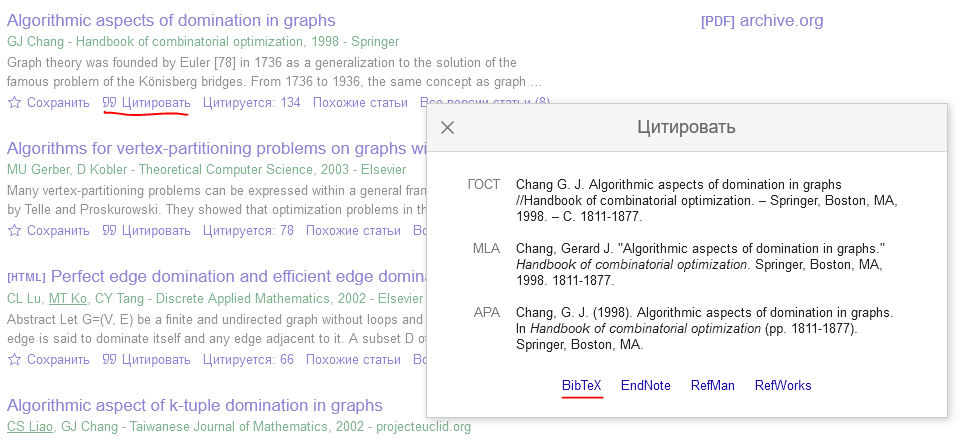
\includegraphics[scale=0.5]{res/img/scholar.png}
    \caption{Как получить bib-цитату на источник в Google Scholar.}
    \label{fig:scholar}
\end{figure}

Ссылка на источник происходит при помощи команды \verb|\cite|: \cite{duportail:alu}. В качестве единственного аргумента указывается идентификатор источника в одном из файлов \verb|*.bib|. Можно указать несколько источников: \cite{duportail:alu, husserl:pd, althusser:iia}, с \verb|\ref| так нельзя. В списке источников отображаются только те источники, на которых есть хотя бы одна ссылка. Если всё-же нужно что бы он там появился без единой ссылки, можно использовать команду \verb|\nocite| в любом месте программы, как под этим абзацем.

Вообще все ссылки кликабельны. Если ссылка неправильная, компилятор выдаст предупреждение, а ссылка будет выглядеть так: \textbf{??}.

\nocite{duportail:alu}
\nocite{althusser:iia}
\nocite{husserl:pd}
\nocite{husserl:sbe}

\chapter{Промышленная экология и безопасность}
\label{cha:bzd}

\section{Протестируем специальные символы.}

И заодно переключение шрифтов.

{\shorthandoff" \texttt{"-{}-* Прямая речь "-{}-{}- <{}<после ,{},тире`{}` неразрывный пробел>{}>}}

{\cyrillicfonttt{\bfseries\itshape\textbackslash{}cyrillicfonttt}
"--* Прямая речь "--- <<после ,,тире`` неразрывный пробел>>.}

{\cyrillicfontsf{\bfseries\itshape\textbackslash{}cyrillicfontsf}
"--* Прямая речь "--- <<после ,,тире`` неразрывный пробел>>.}

{\cyrillicfont{\bfseries\itshape\textbackslash{}cyrillicfont}
"--* Прямая речь "--- <<после ,,тире`` неразрывный пробел>>.}

\blindtext


\backmatter % здесь заканчивается нумерованная часть документа и начинаются ссылки и
            
\Conclusion

В процессе выполнения задания на учебную практику (научно–исследовательскую работу) получены следующие основные результаты.

Изучены рекомендуемые источники и выявлены другие источники. Написан обзор по теме работы. Выбрана концепция разработки устройства отображения.

Кратко описаны используемые при разработке устройства отображения необходимые протоколы и интерфейсы, а именно USB, ULPI, TTL.

Предложена структура устройства отображения, описаны его составные части. Рассмотрена работа устройства отображения. Разработаны необходимые алгоритмы для устройства отображения.

Описание цифровой логической схемы на языке описания аппаратуры заняло \textbf{более 1500 строк}.

Таким образом, была успешно выполнена требуемая разработка устройства отображения, решающего задачи вывода на дисплей графической информации.

В дальнейшем возможно усовершенствование реализованного устройства отображения, например, реализация алгоритмов кодирования или сжатия изображения, что позволит увеличить отображаемое количество кадров в секунду.


 % заключение

\bibliographystyle{ugost2008}
\bibliography{res/references.bib}


\appendix % тут идут приложения

\chapter{Картинки}
\label{cha:appendix1}

\blindtext

\begin{figure}
    \centering
    \includegraphics[scale=3]{example-grid-100x100pt}
    \caption{Картинка в приложении}
\end{figure}


\chapter{Еще картинки}
\label{cha:appendix2}

\blindtext

\begin{figure}
    \centering
    \includegraphics{example-image-golden}
    \caption{Еще одна картинка, ничем не лучше предыдущей. Но надо же как-то заполнить место}
\end{figure}


\end{document}
